\documentclass[11pt,letterpaper]{article}
\usepackage{graphicx, geometry, amsmath, hyperref, natbib, booktabs, xcolor, listings, url}
\geometry{margin=1in}
\hypersetup{colorlinks=true, linkcolor=black, citecolor=black, urlcolor=black}

\title{Compensatory Anti-Correlation in Dependency Distance Sequences:\\A Cross-Linguistic Regularity Beyond Distance Minimization}
\author{}
\date{}

\begin{document}
\maketitle

\begin{abstract}
The dependency distance minimization (DDM) literature treats individual dependencies as statistically independent, analyzing only aggregate sentence-level means or pooled marginal distributions. This paper examines a previously unexplored dimension: the sequential ordering of dependency distances within sentences. We formalize compensatory anti-correlation as excess negative lag-1 autocorrelation of dependency distance sequences relative to grammar-preserving baselines, and measure it across 233 Universal Dependencies treebanks (418,806 sentences of 20 or more non-punctuation tokens, 38 language families). A three-tier baseline hierarchy --- Random Projective Linearization (RPL), Fixed Head-Direction (FHD), and a novel Sibling-Order-Preserving (SOP) baseline --- progressively isolates anti-correlation not attributable to tree structure, head-direction regularities, or co-dependent ordering conventions. Monte Carlo simulation validates estimator properties and confirms that finite-sample bias cancels in the excess measure. A geometric confound analysis on canonical tree topologies demonstrates that the observed anti-correlation is not an artifact of tree geometry. Random-effects meta-analysis yields strongly significant pooled excess autocorrelation at all three tiers (excess-RPL: $-0.131$, $p < 10^{-277}$; excess-FHD: $-0.084$, $p < 10^{-178}$; excess-SOP: $-0.071$, $p < 10^{-225}$), with 99.1\% of treebanks showing negative effects. The anti-correlation is pervasive within treebanks (71--89\% of individual sentences contribute negative excess) and robust to punctuation inclusion, sentence length threshold, and projectivity restrictions. Mixed-effects typological regression with language-family random intercepts reveals that morphological case-marking richness significantly modulates anti-correlation strength ($\beta = 0.080$, $p < 10^{-6}$): languages with richer case systems show weaker compensatory dynamics. Spoken treebanks exhibit stronger anti-correlation than written treebanks (Cohen's $d = -0.83$, $p = 0.001$). These findings establish compensatory anti-correlation as a cross-linguistic regularity in syntactically complex sentences, distinct from both DDM and Uniform Information Density, and provide the first within-sentence statistical signature of the global morphology--word-order trade-off.
\end{abstract}

\section{Introduction}

Dependency distance minimization (DDM) --- the tendency for syntactically related words to appear close together in linear order --- is among the most robust cross-linguistic universals documented in quantitative syntax \citep{Futrell2015, Liu2017, Temperley2018}. Large-scale studies across dozens of languages have demonstrated that mean dependency lengths in natural sentences are significantly shorter than those produced by random linearization baselines \citep{Futrell2015}, that dependency distance distributions follow characteristic two-regime exponential models \citep{Petrini2022}, and that grammar-preserving baselines can modulate the apparent strength of DDM effects \citep{Futrell2020a, Yadav2022}. These findings have motivated information-theoretic accounts of word order as an efficient trade-off between memory cost and predictability \citep{Hahn2021}.

Despite the depth of this literature, a fundamental aspect of dependency distance structure within sentences remains unexplored. All existing studies treat individual dependencies as statistically independent observations, analyzing only aggregate properties: the mean dependency length per sentence \citep{Futrell2015}, the marginal distribution of distances pooled across positions \citep{Petrini2022}, or summary statistics compared against baselines \citep{Futrell2020a, Yadav2022}. No prior work examines the sequential ordering of dependency distances within a sentence --- specifically, whether a long dependency at position $i$ systematically predicts a shorter dependency at position $i+1$, and vice versa.

Detecting such sequential structure is non-trivial for two reasons. First, dependency distance sequences are short --- typically 15 to 40 observations for the long sentences where the phenomenon is most expected --- placing them in a regime where standard autocorrelation estimators exhibit substantial finite-sample bias \citep{Krone2017, Shaman1988}. Second, grammatical regularities in head direction and sibling ordering can produce systematic distance alternation patterns that mimic genuine compensatory dynamics. Disentangling true sequential compensation from structural artifacts requires baselines that control for increasingly fine-grained grammatical regularities \citep{Futrell2020a, Yadav2022}, combined with explicit analysis of geometric confounds inherent in tree topology.

A third challenge arises from the Uniform Information Density (UID) hypothesis \citep{Jaeger2010}, which predicts that speakers distribute information uniformly across sentence positions \citep{Clark2023}. If dependency distance proxies for processing cost, UID could in principle predict the kind of cost-smoothing that appears as anti-correlation. However, dependency distance and surprisal --- UID's primary operationalization --- are empirically uncorrelated in naturalistic reading data \citep{Demberg2008}, establishing that dependency distance anti-correlation cannot be derived from information-rate smoothing alone.

This paper makes four empirical contributions. First, we demonstrate that within-sentence dependency distance sequences exhibit significant negative lag-1 autocorrelation beyond what grammar-preserving baselines predict, establishing compensatory anti-correlation as a cross-linguistic regularity across 233 Universal Dependencies treebanks covering 38 language families and 418,806 long sentences. Second, we validate the measurement methodology through Monte Carlo simulation confirming bias cancellation in the excess measure, and through a geometric confound analysis on canonical tree topologies (star, caterpillar, balanced, random projective) demonstrating that the observed pattern is not an artifact of tree geometry. Third, we show that the effect survives a three-tier baseline hierarchy --- RPL, Fixed Head-Direction (FHD), and a novel Sibling-Order-Preserving (SOP) baseline --- with monotonic attenuation ($-0.131 \to -0.084 \to -0.071$), confirming that the anti-correlation partially but not fully reflects grammatical ordering conventions. Fourth, we show that morphological case-marking richness significantly predicts anti-correlation strength ($\beta = 0.080$, $p < 10^{-6}$), providing the first within-sentence statistical signature of the global trade-off between morphological complexity and word-order rigidity \citep{Bentz2017}.

\subsection{Summary of Contributions}

\begin{itemize}
  \item \textbf{Empirical finding}: Compensatory anti-correlation (excess negative lag-1 autocorrelation) is a pervasive cross-linguistic regularity in long sentences, with pooled excess-RPL $= -0.131$ ($p < 10^{-277}$) across 233 treebanks (Section~\ref{sec:results}).
  \item \textbf{Methodological validation}: Monte Carlo simulation, bias-cancellation analysis, and geometric confound analysis on canonical trees confirm measurement validity (Section~\ref{sec:validation}).
  \item \textbf{Three-tier baseline hierarchy}: The novel SOP baseline isolates anti-correlation beyond all observed grammatical ordering conventions; the effect survives at all tiers (Section~\ref{sec:main_meta}).
  \item \textbf{Typological modulation}: Case-marking richness weakens anti-correlation; spoken treebanks show stronger effects than written treebanks (Section~\ref{sec:typological}).
  \item \textbf{Robustness}: Results hold across punctuation inclusion/exclusion, sentence length thresholds, and projectivity restrictions (Section~\ref{sec:robustness}).
\end{itemize}

\section{Related Work}

\subsection{Dependency Distance Minimization}

The foundational result in this area is \citet{Futrell2015}'s demonstration that mean dependency lengths across 37 languages are significantly shorter than RPL baselines, establishing DDM as a cross-linguistic universal. \citet{Liu2017} provided early large-scale evidence across 20 languages, proposing a mean dependency distance threshold of approximately 3 words. \citet{Temperley2018} offered a comprehensive review of DDM evidence from corpora, experiments, and computational models. Subsequent work refined the baseline methodology: \citet{Futrell2020a} dissociated grammar-level from usage-level word-order optimization across 53 languages, while \citet{Yadav2022} challenged DDM universality by showing that some languages do not minimize dependency length relative to grammar-preserving baselines. These studies established increasingly sophisticated baselines but focused exclusively on aggregate dependency length measures, not on the sequential ordering of distances within sentences.

\subsection{Dependency Distance Distributions}

\citet{Petrini2022} discovered that the marginal distribution of dependency distances follows a two-regime exponential model with a break-point at 4--5 words, consistent across 20 languages. This distributional characterization is complementary to but distinct from the present work, which examines sequential ordering within sentences rather than pooled distributions.

\subsection{Uniform Information Density}

The UID hypothesis, formulated by \citet{Jaeger2010}, holds that speakers prefer utterances distributing information uniformly across the signal. \citet{Meister2021} explored multiple operationalizations of UID, finding the strongest trend is regression towards a mean surprisal at the language level. \citet{Clark2023} tested UID cross-linguistically in 10 languages using counterfactual word-order baselines, finding that SVO languages show greater uniformity than reversed orders. \citet{Tsipidi2024} challenged UID at the discourse level, proposing a Structured Context Hypothesis in which speakers modulate information rate based on hierarchical discourse structure.

The present work differs from UID research in three key respects\footnote{Code: \url{https://github.com/AMGrobelnik/ai-invention-c3cfa4-sequential-dependency-distance-anti-corr/tree/main/research_iter3_uid_vs_dd_novel}}. First, UID operates on surprisal (information rate), whereas compensatory anti-correlation operates on structural dependency distance. \citet{Demberg2008} showed that these two quantities are empirically uncorrelated in naturalistic reading data: dependency-based integration cost does not predict reading times for arbitrary words, while surprisal does. This uncorrelatedness means that anti-correlation patterns in dependency distance sequences cannot be derived from surprisal smoothing, even under the strongest UID interpretation. Second, UID baselines (reversed, shuffled orders) destroy both grammatical structure and usage-level patterns simultaneously \citep{Clark2023}, whereas the RPL/FHD/SOP hierarchy progressively controls for grammatical regularities at increasing fidelity. Third, the prediction that case-marking richness modulates anti-correlation strength has no analogue in UID theory --- no existing UID framework predicts that information-rate smoothing should vary with morphological complexity.

\subsection{Morphological Complexity and Word Order}

\citet{Bentz2017} demonstrated a global inverse correlation between word-order rigidity and morphological complexity across approximately 1,200 languages, establishing a macro-typological trade-off. \citet{Hahn2021} formalized word order optimization as a memory-surprisal trade-off. \citet{Futrell2020b} derived dependency locality effects from information theory via lossy-context surprisal, treating dependency distance and surprisal as complementary phenomena. These global patterns motivate the present prediction that morphological case-marking modulates within-sentence compensatory dynamics, but no prior work has identified a specific within-sentence statistical signature of the global complexity trade-off.

\subsection{Spoken vs.\ Written Syntax and Linearization Algorithms}

\citet{Dobrovoljc2025} compared syntactic structure inventories between spoken and written UD treebanks, finding that spoken corpora contain fewer and less diverse structures, motivating the present spoken/written comparison. The RPL baseline originates from \citet{Gildea2007, Gildea2010}, with \citet{AlemanyPuig2022} providing linear-time algorithms for expected dependency lengths under random projective linearizations. The present work extends this foundation with two additional baseline tiers.

\subsection{Autocorrelation Estimation in Short Series}

The challenge of estimating autocorrelation from short sequences is well-studied in clinical single-case design methodology. \citet{Arnau2001} proposed the r1-prime polynomial bias-correction estimator for series with fewer than 50 observations. \citet{Krone2017} compared AR(1) estimators across series lengths 10--100, finding that power falls below 80\% for all methods when series length is under 50 and autocorrelation magnitude is below 0.40. \citet{Shaman1988} derived analytical $O(1/T)$ bias formulas for autoregressive estimators. \citet{Dou2026} analytically demonstrated the causes and consequences of small-sample OLS bias in AR(1) models. These findings from clinical methodology directly address the statistical challenges inherent in analyzing dependency distance sequences.

\section{Methods}

\subsection{Dependency Distance Sequences}

For a sentence with tokens at positions $1, 2, \ldots, n$, we define the dependency distance sequence as the ordered series $DD_1, DD_2, \ldots, DD_m$ where $DD_i = |i - \text{head}(i)|$ for each non-root, non-punctuation token $i$ in linear order\footnote{Code: \url{https://github.com/AMGrobelnik/ai-invention-c3cfa4-sequential-dependency-distance-anti-corr/tree/main/dataset_iter1_ud_dep_extract}}. Punctuation tokens (those with dependency relation label \texttt{punct}) are excluded from the sequence, as punctuation in Universal Dependencies typically attaches to nearby words with very short distances at predictable positions (e.g., sentence-final periods), creating artificial sequential patterns that could confound autocorrelation estimates. The sequence length $m$ equals the number of content-bearing tokens minus one (the root). We treat this sequence as a discrete time series and compute its lag-1 autocorrelation:
\begin{equation}
r_1 = \frac{\sum_{t=1}^{m-1}(DD_t - \overline{DD})(DD_{t+1} - \overline{DD})}{\sum_{t=1}^{m}(DD_t - \overline{DD})^2}
\end{equation}
A significantly negative $r_1$ indicates compensatory anti-correlation: long dependencies tend to be followed by shorter ones, and vice versa. The primary analysis requires $m \geq 20$ non-punctuation tokens; robustness checks use $m \geq 15$.

\subsection{Three-Tier Baseline Hierarchy}

To determine whether observed anti-correlation exceeds what grammatical structure alone predicts, we construct three baselines per sentence in a hierarchy of increasing grammatical fidelity\footnote{Code: \url{https://github.com/AMGrobelnik/ai-invention-c3cfa4-sequential-dependency-distance-anti-corr/tree/main/research_iter1_dd_baselines}}.

\textbf{Tier 1: Random Projective Linearization (RPL).} Following \citet{Gildea2007, Gildea2010} as adopted by \citet{Futrell2015}, RPL randomly assigns each dependent to either the left or right of its head, randomly orders dependents within each side, and recurses through the tree, maintaining projectivity. For each sentence, 100 random linearizations are generated. RPL controls for tree shape while randomizing all ordering decisions.

\textbf{Tier 2: Fixed Head-Direction (FHD).} Building on the fixed-word-order baselines of \citet{Futrell2020a}, FHD fixes the head direction (initial or final) for each dependency relation type to the majority pattern observed across the treebank. Dependents on the same side of the head are randomly ordered. FHD controls for systematic head-direction regularities while preserving residual randomness in sibling ordering.

\textbf{Tier 3: Sibling-Order-Preserving (SOP).} SOP is a novel baseline that extends FHD by additionally fixing the relative linear ordering of all co-dependents sharing the same head\footnote{Code: \url{https://github.com/AMGrobelnik/ai-invention-c3cfa4-sequential-dependency-distance-anti-corr/tree/main/dataset_iter1_ud_grammar_prof}}. For each head node, the conditioning key consists of the head's part-of-speech tag and the multiset of dependency relation types of its dependents. The majority ordering template is extracted from treebank statistics with a minimum count threshold of 5 occurrences. When a configuration falls below the threshold, SOP falls back to FHD behavior. SOP captures sibling-ordering regularities such as subject-before-object in English that can produce systematic distance alternation surviving the FHD baseline.

\begin{figure}[!htbp]
  \centering
  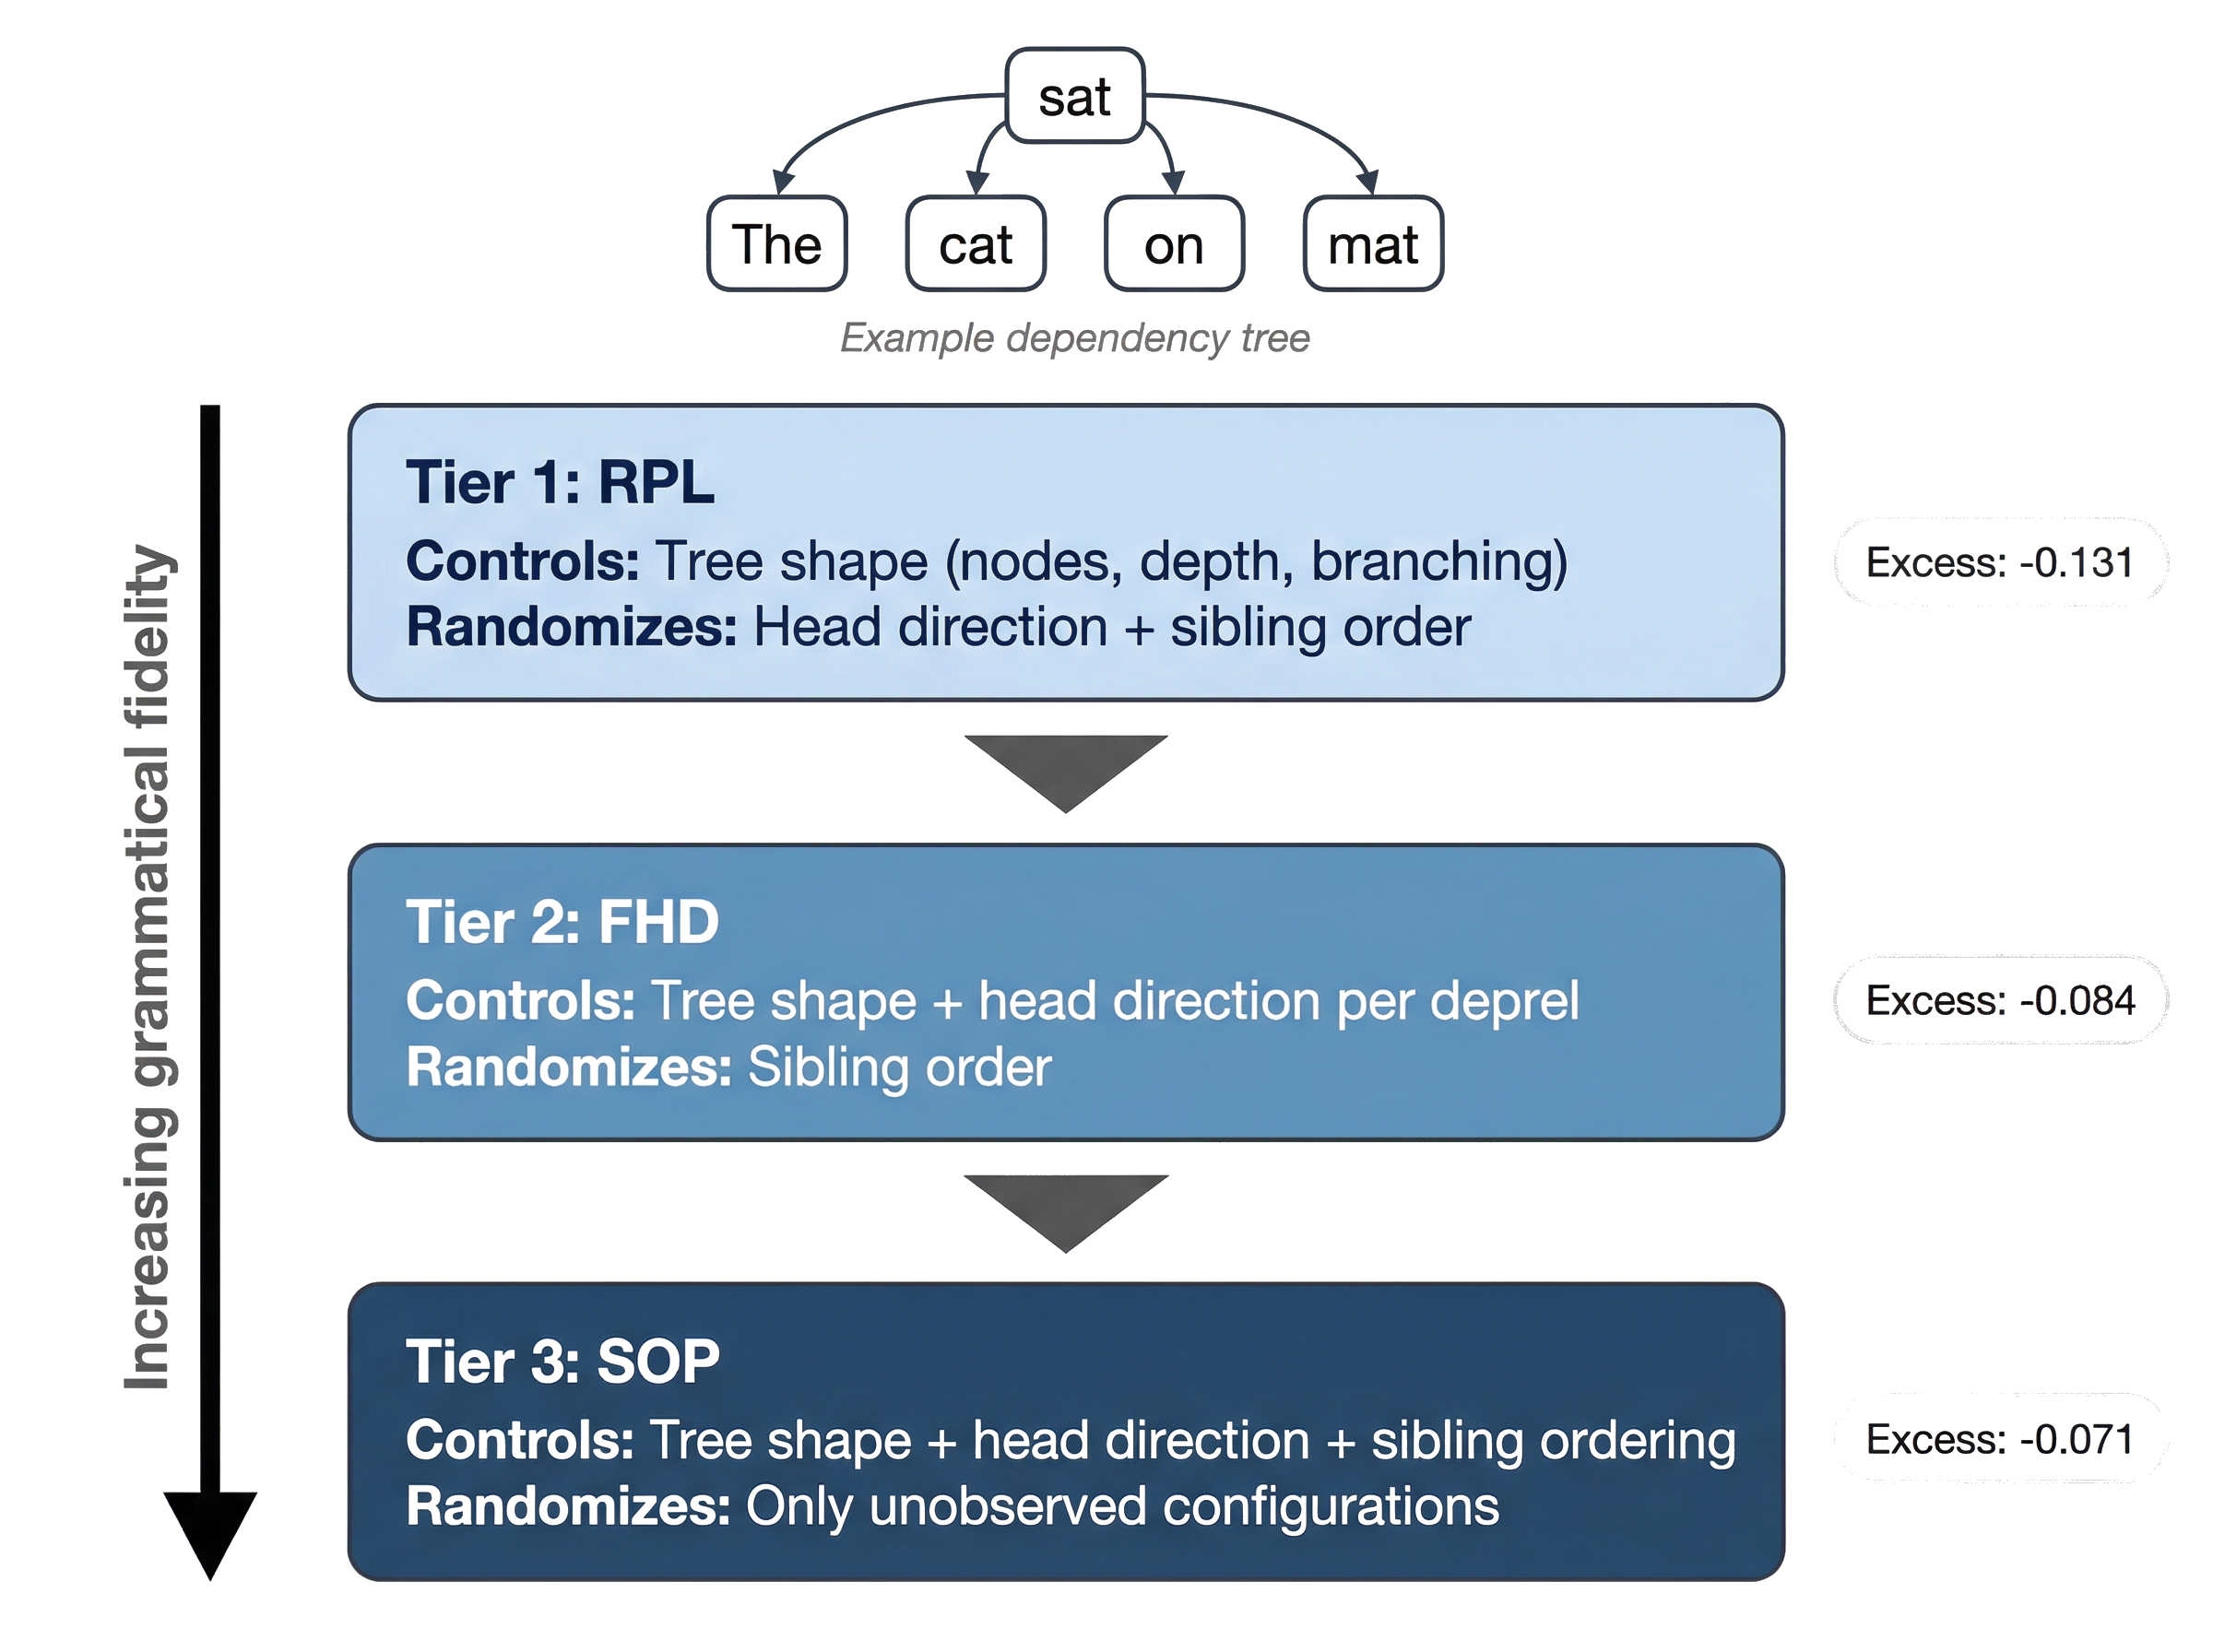
\includegraphics[width=0.92\textwidth,keepaspectratio]{figures/fig_1_v0.png}
  \caption{The three-tier baseline hierarchy for isolating compensatory anti-correlation. Each tier adds grammatical constraints: RPL controls for tree shape, FHD additionally fixes head direction per relation type, and the novel SOP baseline additionally fixes relative ordering of co-dependents. Excess autocorrelation is the difference between observed and baseline lag-1 autocorrelation at each tier.}
  \label{fig:baseline_hierarchy}
\end{figure}

For each sentence and each baseline tier, excess autocorrelation is defined as:
\begin{equation}
\text{excess-}B = r_1^{\text{observed}} - \overline{r_1^B}
\end{equation}
where $\overline{r_1^B}$ is the mean lag-1 autocorrelation across the baseline linearizations at tier $B \in \{\text{RPL}, \text{FHD}, \text{SOP}\}$. A significantly negative excess value indicates anti-correlation beyond what the baseline's grammatical constraints explain. Figure~\ref{fig:baseline_hierarchy} illustrates the three-tier hierarchy.

\subsection{Bias-Corrected Estimation and Geometric Confound Analysis}

Standard autocorrelation estimators exhibit systematic negative bias in short series, with $E[r_1] \approx \rho - (1 + 3\rho)/n$ for AR(1) processes of length $n$ \citep{Shaman1988}. For dependency distance sequences of 20--40 tokens, this bias can reach 0.05 in magnitude. However, because the excess measure computes the difference between observed and baseline estimates of equal sequence length, finite-sample bias that is similar for both cancels in the subtraction \citep{Krone2017, Dou2026}. This bias-cancellation property makes the standard $r_1$ estimator optimal for excess computation despite its absolute bias, since $r_1$ has the lowest variance among common estimators \citep{Krone2017}. We validate this property through Monte Carlo simulation (Section~\ref{sec:validation}).

A separate concern is that tree geometry alone may produce systematic anti-correlation that persists through the baseline hierarchy. A token far from its head (high DD) may be surrounded by tokens in the same subtree that are close to their own heads (low DD), creating inherent anti-correlation from topology rather than a compensatory mechanism. To address this confound, we conduct a geometric null model analysis on four canonical tree types --- star graphs, caterpillar trees, balanced binary trees, and random Galton-Watson projective trees --- computing excess autocorrelation for each under RPL baselines. If the canonical trees produce near-zero or positive excess, the observed negative excess in real data cannot be attributed to geometric artifacts.

\subsection{Projectivity Stratification}

Non-projective sentences contain crossing dependency arcs that can produce distinctive distance patterns no projective linearization can replicate. To prevent this from biasing excess estimates, we conduct the primary analysis on all sentences and report a separate projective-only variant as a robustness check, using projectivity rates from the grammar profiles.

\subsection{Statistical Analysis Framework}

The analysis employs a two-tier statistical framework\footnote{Code: \url{https://github.com/AMGrobelnik/ai-invention-c3cfa4-sequential-dependency-distance-anti-corr/tree/main/research_iter1_autocorr_meta}}.

\textbf{Tier 1: Random-effects meta-analysis.} Per-treebank effect sizes (mean excess autocorrelation and its variance) are pooled using a random-effects meta-analytic model with REML estimation for between-treebank variance \citep{Veroniki2016}. For each baseline level, we report the pooled estimate with 95\% confidence interval, heterogeneity statistics ($I^2$, $\tau^2$), and 95\% prediction intervals. A language-level sensitivity analysis aggregates same-language treebanks before meta-analytic pooling, addressing within-language dependence across multiple treebanks of the same language.

\textbf{Tier 2: Mixed-effects typological regression.} Treebank-level excess autocorrelation is modeled as a function of typological predictors with language family as a random intercept:
\begin{equation}
\text{excess}_{t} = \beta_0 + \beta_1 \cdot \text{modality} + \beta_2 \cdot \text{case\_richness} + \beta_3 \cdot \text{mean\_length} + u_{\text{family}(t)} + \epsilon_t
\end{equation}
Case-marking richness is measured on a continuous scale combining WALS Chapter 49A (Number of Cases) \citep{Dryer2013} and UD-derived proportions of tokens bearing morphological Case features\footnote{Code: \url{https://github.com/AMGrobelnik/ai-invention-c3cfa4-sequential-dependency-distance-anti-corr/tree/main/dataset_iter1_ud_typology_tab}}. Cross-source consistency is validated via Spearman rank correlation (appropriate for ordinal vs.\ continuous data). Modality (spoken vs.\ written) is identified from UD treebank metadata, with covariates for mean sentence length to control for structural differences between modalities.

\section{Results}
\label{sec:results}

\subsection{Phase 1: Measurement Validation}
\label{sec:validation}

\subsubsection{Monte Carlo Estimator Comparison}

Monte Carlo simulation of synthetic AR(1) sequences across six lengths ($n \in \{10, 15, 20, 25, 30, 40\}$) and 17 true autocorrelation values ($\rho \in \{-0.40, \ldots, 0.40\}$) with 10,000 replications per cell compared three estimators: standard $r_1$, the Marriott-Pope analytical correction, and maximum likelihood estimation\footnote{Code: \url{https://github.com/AMGrobelnik/ai-invention-c3cfa4-sequential-dependency-distance-anti-corr/tree/main/experiment_iter3_mc_geometry}}.

At $n = 20$ (the primary analysis threshold), the standard $r_1$ estimator exhibits moderate negative bias that increases with the magnitude of the true autocorrelation: bias $= -0.013$ at $\rho = -0.20$, bias $= -0.025$ at $\rho = -0.15$, and bias $= -0.048$ at $\rho = 0.00$. The corrected estimator reduces absolute bias (e.g., bias $= 0.006$ at $\rho = -0.20$) but at substantially higher RMSE ($0.230$ vs.\ $0.200$). No individual estimator achieves 80\% power at any sequence length $\leq 40$ for any tested autocorrelation magnitude, confirming that meta-analytic pooling across sentences is essential for adequate statistical power \citep{Krone2017}.

The bias-cancellation hypothesis was confirmed empirically: when two independent AR(1) sequences of equal length are generated and their $r_1$ values differenced, the mean excess is near zero regardless of the true $\rho$ (e.g., at $n = 20$, $\rho = -0.20$: mean excess $= -0.011$, with zero contained in the 95\% CI). At $n = 30$, $\rho = -0.20$: mean excess $= 0.007$. This validates using the standard $r_1$ estimator for excess computation, as its lower variance ($\text{RMSE} = 0.200$ vs.\ $0.230$ for the corrected estimator at $n = 20$) translates to greater statistical power in the meta-analysis without introducing systematic bias in the excess measure.

\begin{figure}[!htbp]
  \centering
  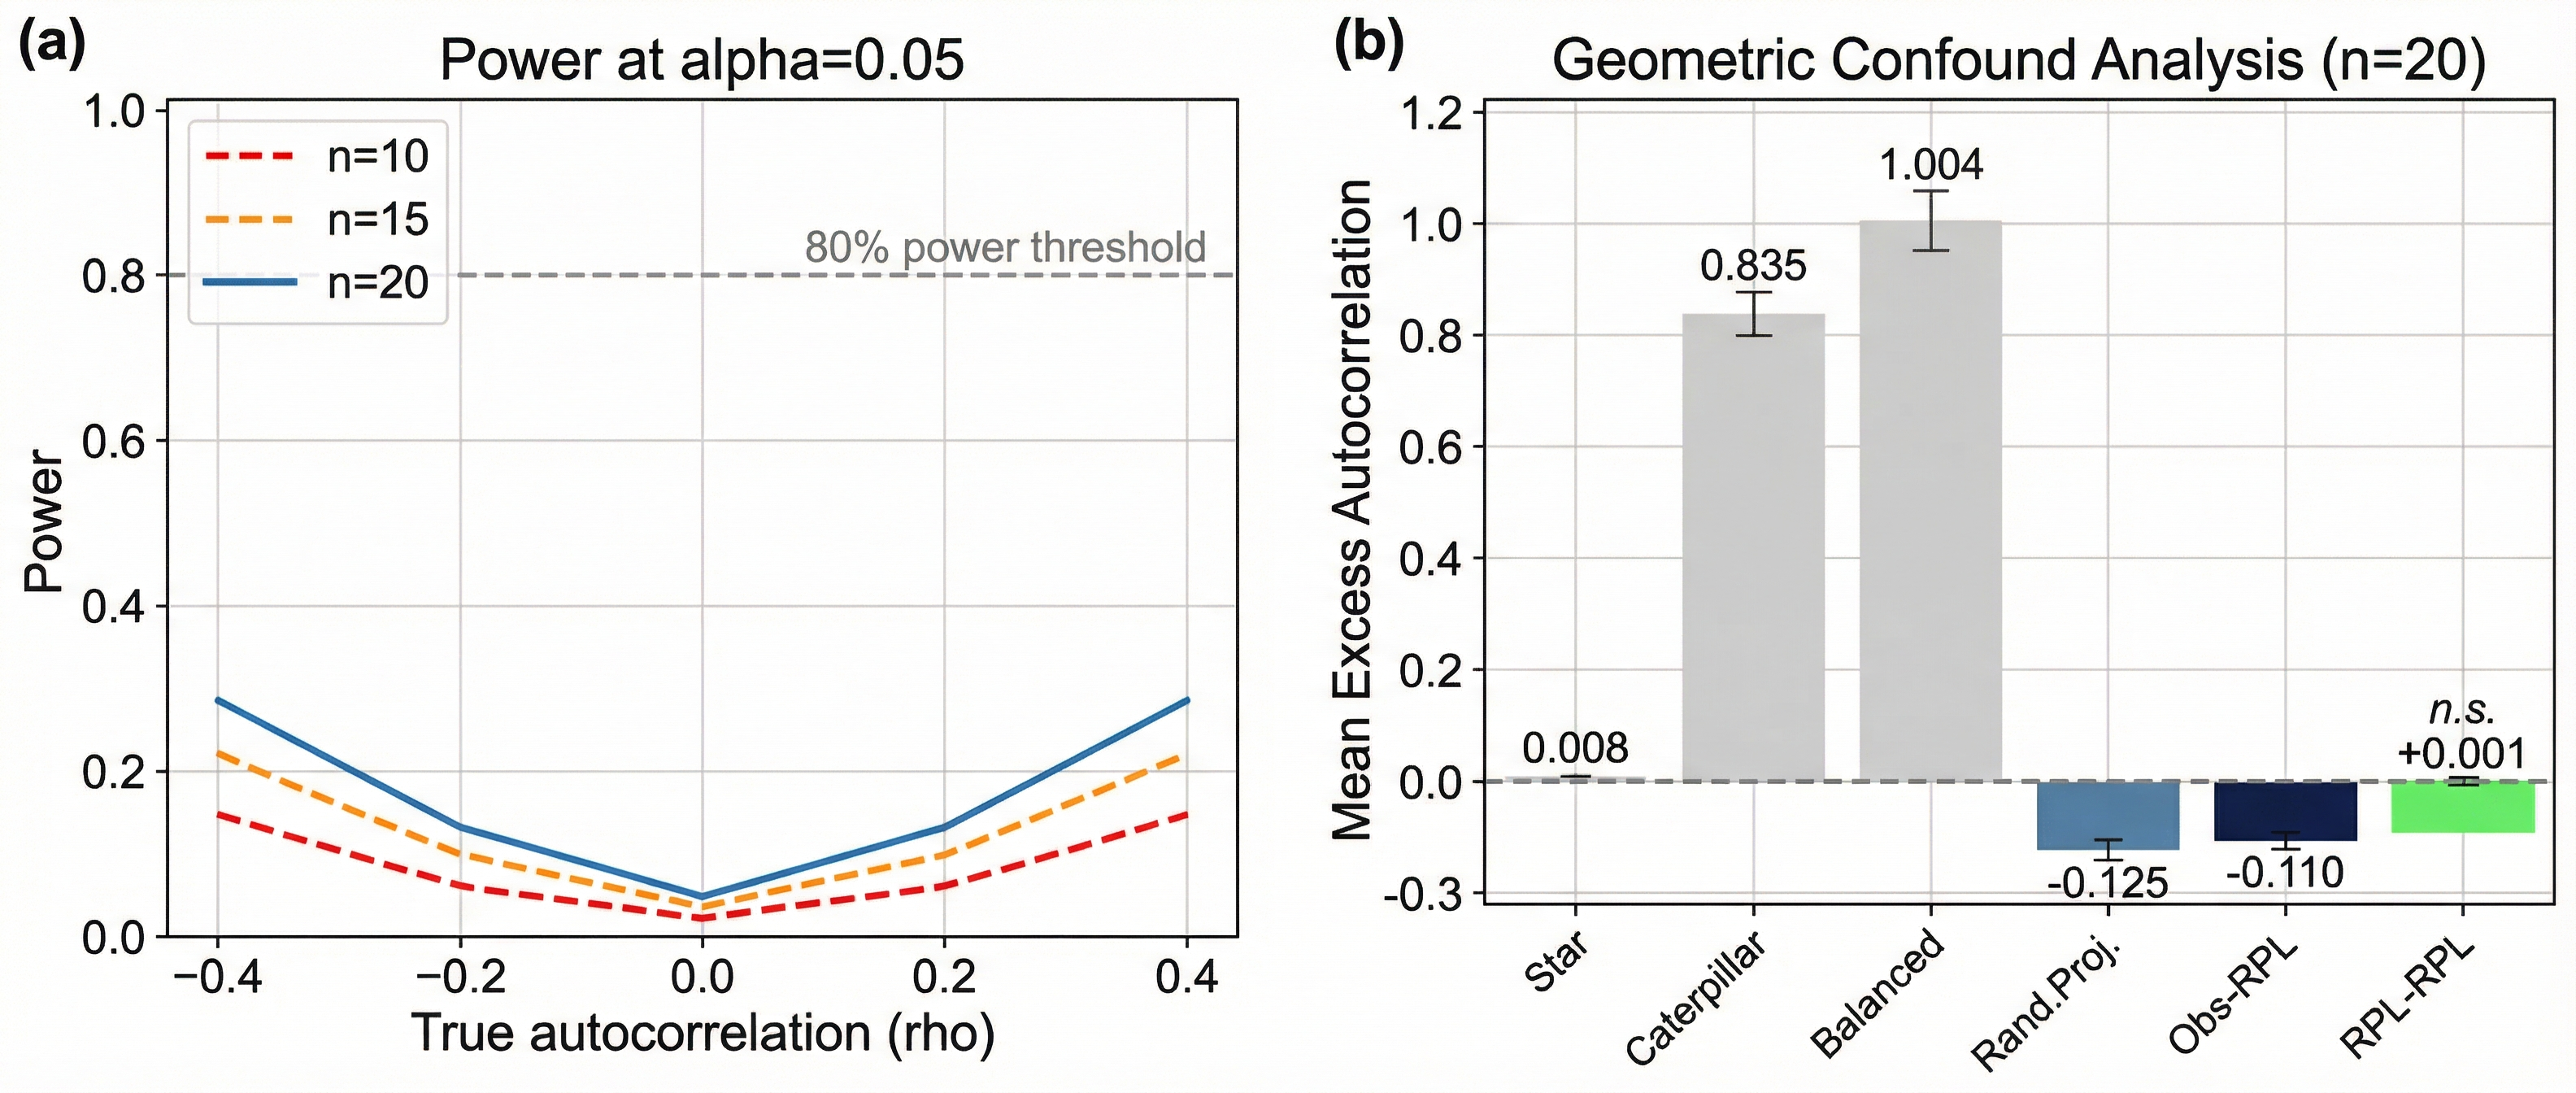
\includegraphics[width=0.92\textwidth,keepaspectratio]{figures/fig_2_v0.png}
  \caption{Left: Power curves for the standard $r_1$ estimator at sequence lengths $n \in \{10, 15, 20\}$ across true autocorrelation values $\rho \in [-0.40, 0.40]$, showing that no individual sequence achieves 80\% power. Right: Geometric confound analysis on canonical tree types ($n = 20$, 500 trees each). Star, caterpillar, and balanced trees produce zero or positive excess-RPL; only random projective trees produce negative excess ($-0.125$), but RPL-vs-RPL control confirms this excess is zero under the null ($+0.001$, $p = 0.23$).}
  \label{fig:monte_carlo}
\end{figure}

\subsubsection{Geometric Confound Analysis}

To determine whether tree geometry alone produces negative excess autocorrelation that could masquerade as compensatory dynamics, we analyzed four canonical tree types at sizes $n \in \{20, 30, 40\}$ with 500 trees each.

Star graphs (all tokens depend on a single root) and caterpillar trees (linear chains) produce near-zero or strongly positive excess autocorrelation: star graphs yield mean excess of $+0.008$ ($n = 20$) to $+0.001$ ($n = 40$), while caterpillar trees yield $+0.835$ to $+0.850$ and balanced binary trees yield $+1.004$ to $+1.016$. None of these canonical topologies produce negative excess, demonstrating that the RPL baseline absorbs geometric anti-correlation from these structures.

Random projective trees generated via Galton-Watson processes produce negative excess ($-0.125$ at $n = 20$, $-0.119$ at $n = 40$), with 84--91\% of individual trees showing negative excess. However, a critical control analysis on 2,000 real UD sentences establishes that this negative excess is not a geometric artifact: when one RPL linearization is compared against another RPL linearization of the same tree (RPL-vs-RPL), the mean excess is $+0.001$ ($p = 0.23$, not significant), confirming the RPL null model is valid. In contrast, observed linearizations vs.\ RPL baselines yield mean excess $= -0.110$ ($p < 10^{-136}$), and randomly shuffled token-order vs.\ RPL yields only $-0.020$ ($p < 10^{-5}$). The difference between observed and shuffled excess is $-0.091$ ($p < 10^{-51}$), demonstrating that the sequential ordering of real sentences --- not tree geometry --- drives the anti-correlation. Figure~\ref{fig:monte_carlo} summarizes these validation results.

\subsection{Phase 2--3: Excess Autocorrelation Across 233 Treebanks}
\label{sec:main_meta}

\subsubsection{Main Meta-Analytic Results}

The core analysis processes 233 qualifying treebanks from Universal Dependencies v2.17 \citep{Nivre2020} containing at least 50 sentences with $\geq 20$ non-punctuation tokens, totaling 418,806 sentences across 38 language families\footnote{Code: \url{https://github.com/AMGrobelnik/ai-invention-c3cfa4-sequential-dependency-distance-anti-corr/tree/main/experiment_iter3_dd_autocorr_exp}}.

Random-effects meta-analysis with REML estimation yields strongly significant negative pooled excess autocorrelation at all three baseline tiers, with monotonic attenuation through the hierarchy:

\begin{table}[!htbp]
\centering
\caption{Random-effects meta-analytic pooled estimates of excess autocorrelation across 233 treebanks. All estimates are significantly negative ($p < 10^{-170}$). The hierarchy shows monotonic attenuation as baselines incorporate more grammatical structure.}
\label{tab:main_results}
\begin{tabular}{lcccccc}
\toprule
\textbf{Measure} & \textbf{Pooled} & \textbf{95\% CI} & \textbf{$p$} & \textbf{$I^2$} & \textbf{Pred.\ Int.} & \textbf{\% Neg.} \\
\midrule
Excess-RPL & $-0.131$ & $[-0.139, -0.124]$ & $< 10^{-277}$ & 0.983 & $[-0.240, -0.022]$ & 99.1\% \\
Excess-FHD & $-0.084$ & $[-0.090, -0.079]$ & $< 10^{-178}$ & 0.972 & $[-0.171, +0.002]$ & 98.3\% \\
Excess-SOP & $-0.071$ & $[-0.075, -0.067]$ & $< 10^{-225}$ & 0.942 & $[-0.134, -0.008]$ & 99.1\% \\
\bottomrule
\end{tabular}
\end{table}

The attenuation from excess-RPL ($-0.131$) to excess-FHD ($-0.084$) indicates that approximately 36\% of the RPL-level anti-correlation is attributable to head-direction regularities. The further attenuation to excess-SOP ($-0.071$) indicates that sibling-ordering conventions account for an additional 10\% of the original effect. Crucially, the remaining excess-SOP of $-0.071$ is highly significant ($p < 10^{-225}$), with the 95\% prediction interval entirely below zero ($[-0.134, -0.008]$), confirming that the compensatory pattern cannot be explained by any observed grammatical ordering convention.

The high $I^2$ values (0.942--0.983) indicate substantial between-treebank heterogeneity, expected given the typological diversity of the sample. The prediction intervals characterize the expected range of effects in future treebanks: even at the SOP level, a new treebank is predicted to show negative excess with high probability.

\begin{figure}[!htbp]
  \centering
  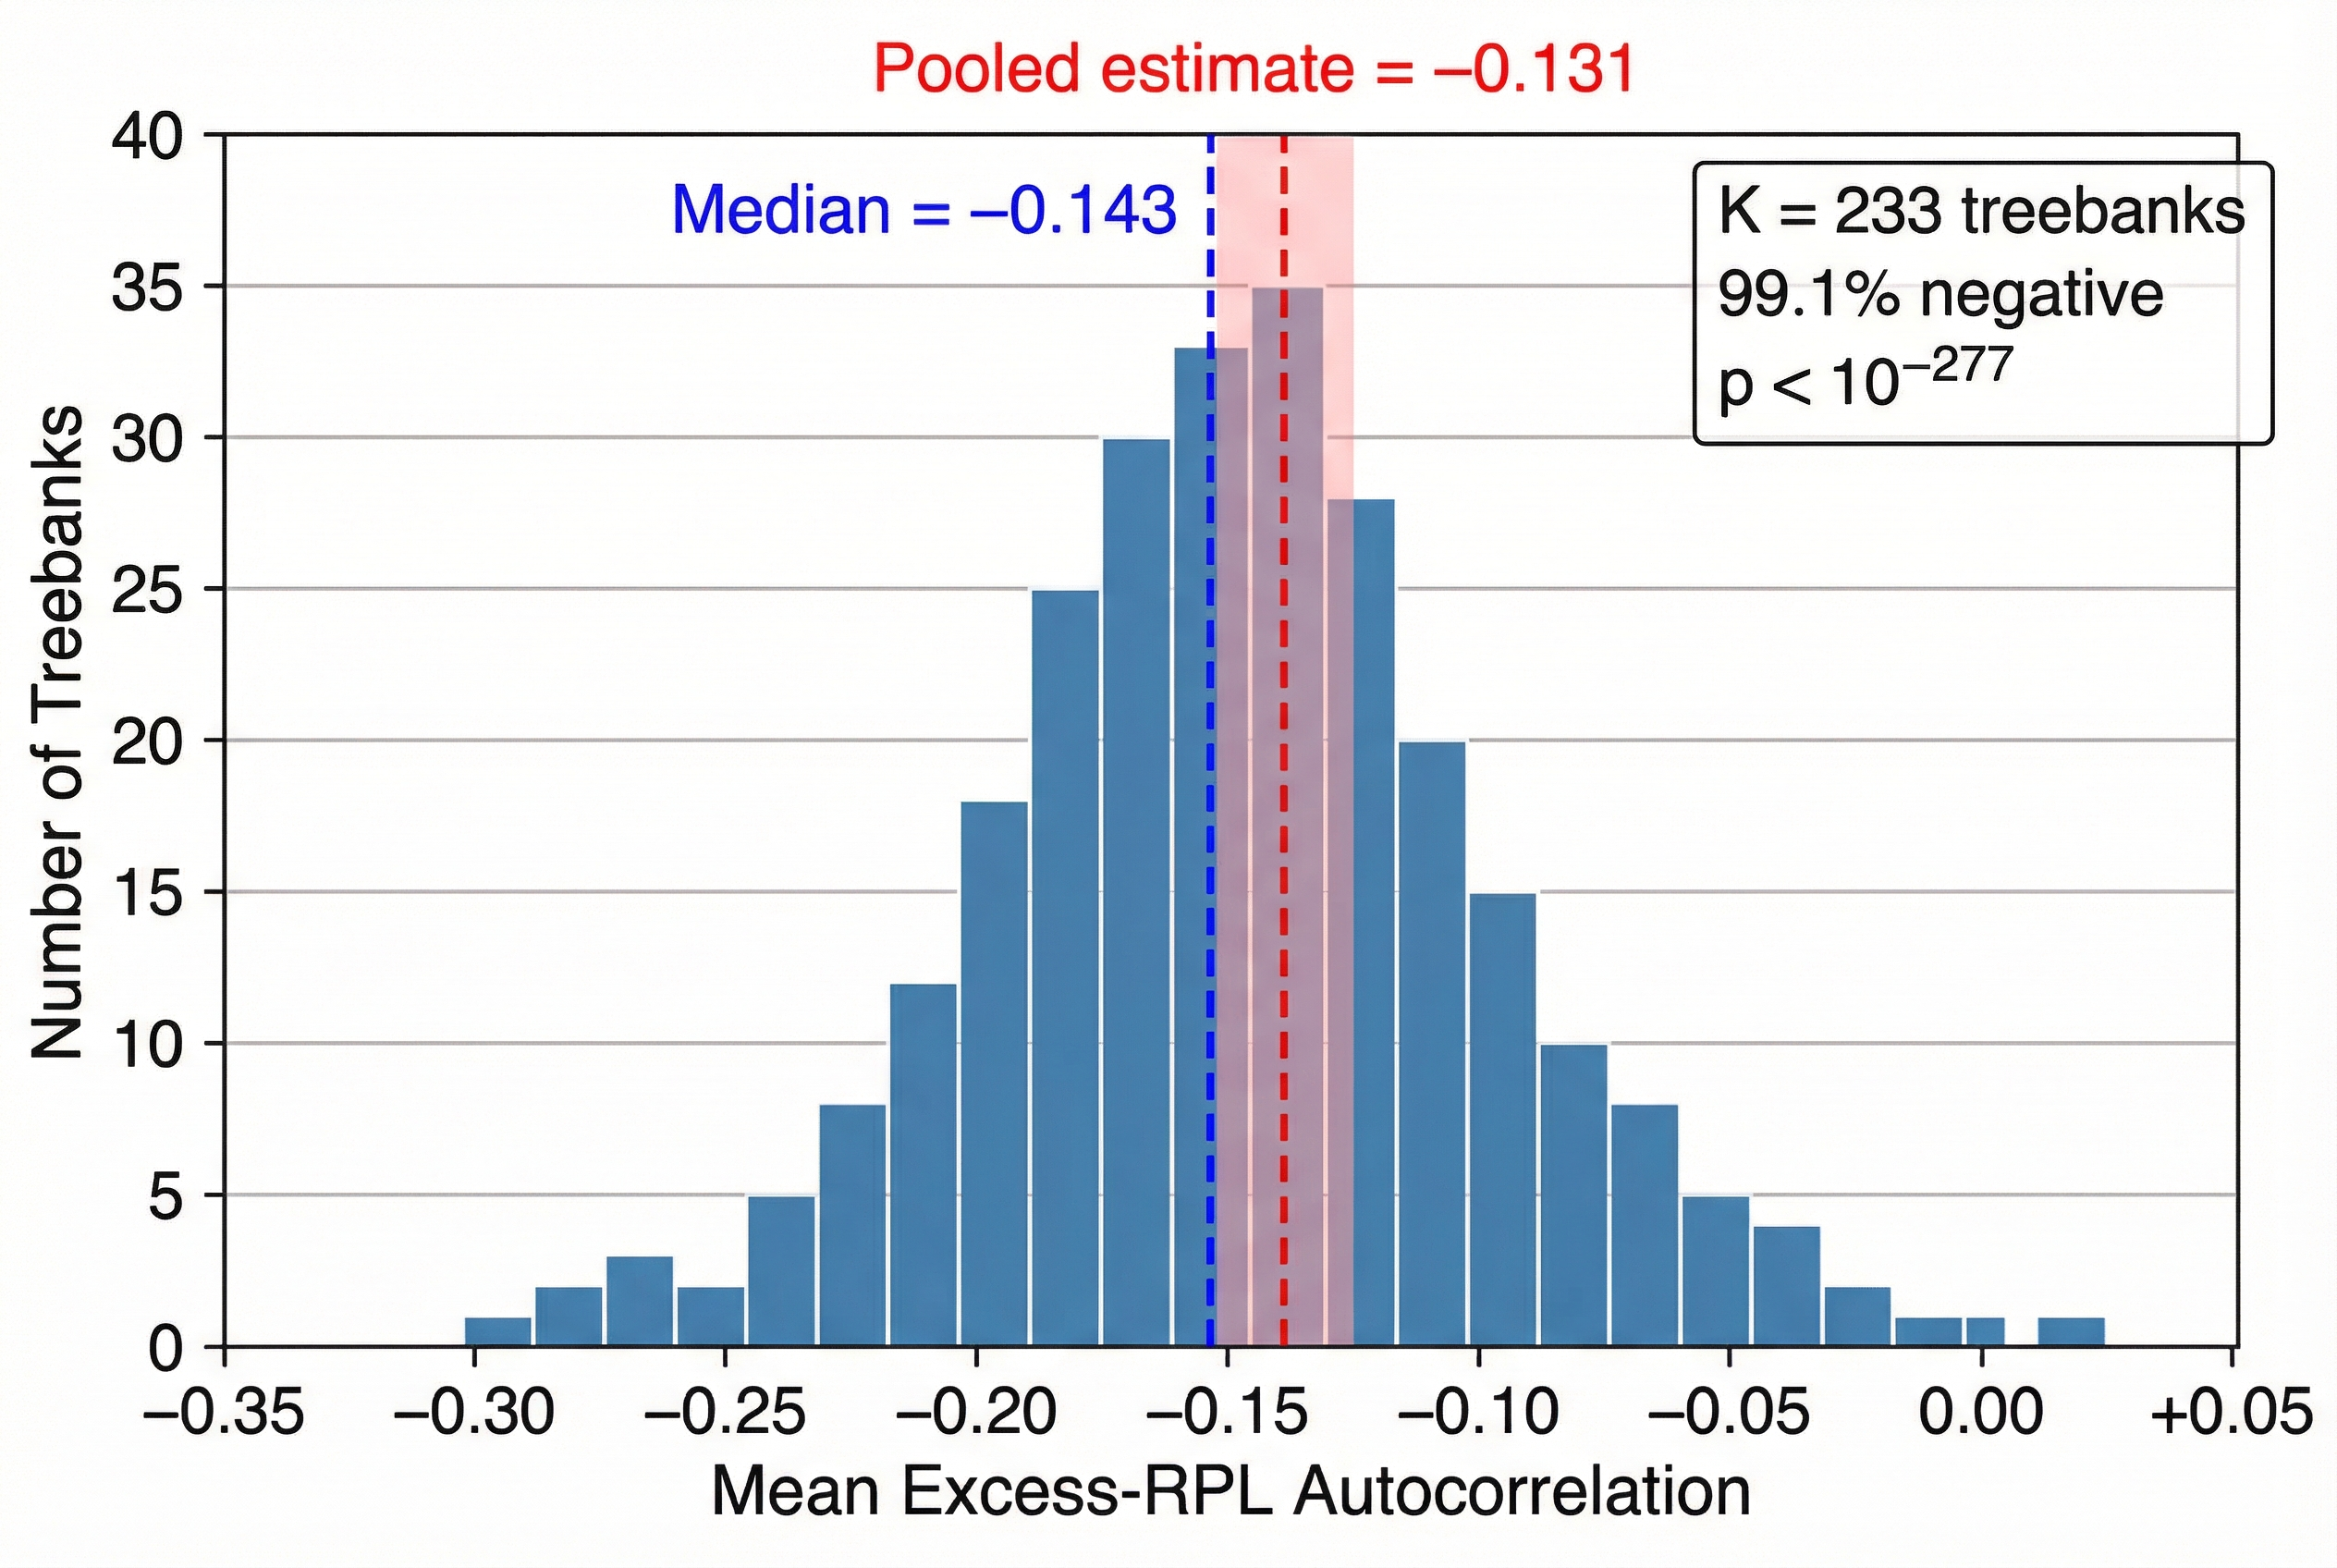
\includegraphics[width=0.92\textwidth,keepaspectratio]{figures/fig_3_v0.png}
  \caption{Histogram of per-treebank mean excess-RPL autocorrelation across 233 qualifying treebanks from Universal Dependencies v2.17. The pooled random-effects meta-analytic estimate is $-0.131$ (vertical dashed red line). 99.1\% of treebanks (231/233) show negative excess. The distribution spans from approximately $-0.30$ to $+0.02$, with median $-0.143$.}
  \label{fig:histogram}
\end{figure}

Figure~\ref{fig:histogram} shows the distribution of per-treebank excess-RPL across all 233 treebanks, demonstrating the near-universality of the negative excess pattern.

\subsubsection{Within-Treebank Pervasiveness}

The treebank-level effects are not driven by extreme sentences but reflect pervasive within-sentence patterns\footnote{Code: \url{https://github.com/AMGrobelnik/ai-invention-c3cfa4-sequential-dependency-distance-anti-corr/tree/main/experiment_iter3_rpl_diagnostics}}. Across 30 strategically selected treebanks spanning diverse language families (all significant at $p < 0.001$), the proportion of individual sentences contributing negative excess-RPL ranges from 71.5\% (German de\_hdt, 77,077 sentences) to 88.9\% (Russian ru\_syntagrus, 30,145 sentences), with Czech cs\_pdtc at 88.0\% (68,065 sentences). The median proportion across the 30 treebanks exceeds 75\%, confirming that the effect is pervasive rather than driven by a structural subtype.

Structural subtype analysis reveals that the bottom-10\% sentences (those with the most negative excess) tend to have lower maximum dependency distance than the full population in 28 of 30 treebanks, suggesting that compensatory dynamics are strongest when no single very long dependency dominates the sentence.

\subsubsection{Language-Level Sensitivity}

To address within-language dependence across multiple treebanks of the same language, we aggregate all treebanks sharing a language before meta-analytic pooling\footnote{Code: \url{https://github.com/AMGrobelnik/ai-invention-c3cfa4-sequential-dependency-distance-anti-corr/tree/main/experiment_iter3_robustness_4_va}}. The language-level pooled estimate is $-0.133$ ($p < 10^{-188}$, $K = 114$ languages), virtually identical to the treebank-level estimate, confirming that the result is not inflated by within-language dependence. Within-language consistency is high: for instance, English treebanks (en\_childes: $-0.278$, en\_eslspok: $-0.246$, en\_gum: $-0.236$), Czech treebanks (cs\_cac: $-0.213$, cs\_pdtc: $-0.194$), and Finnish treebanks (fi\_ftb: $-0.230$, fi\_tdt: $-0.238$) show closely matched effects across treebanks of the same language.

\begin{figure}[!htbp]
  \centering
  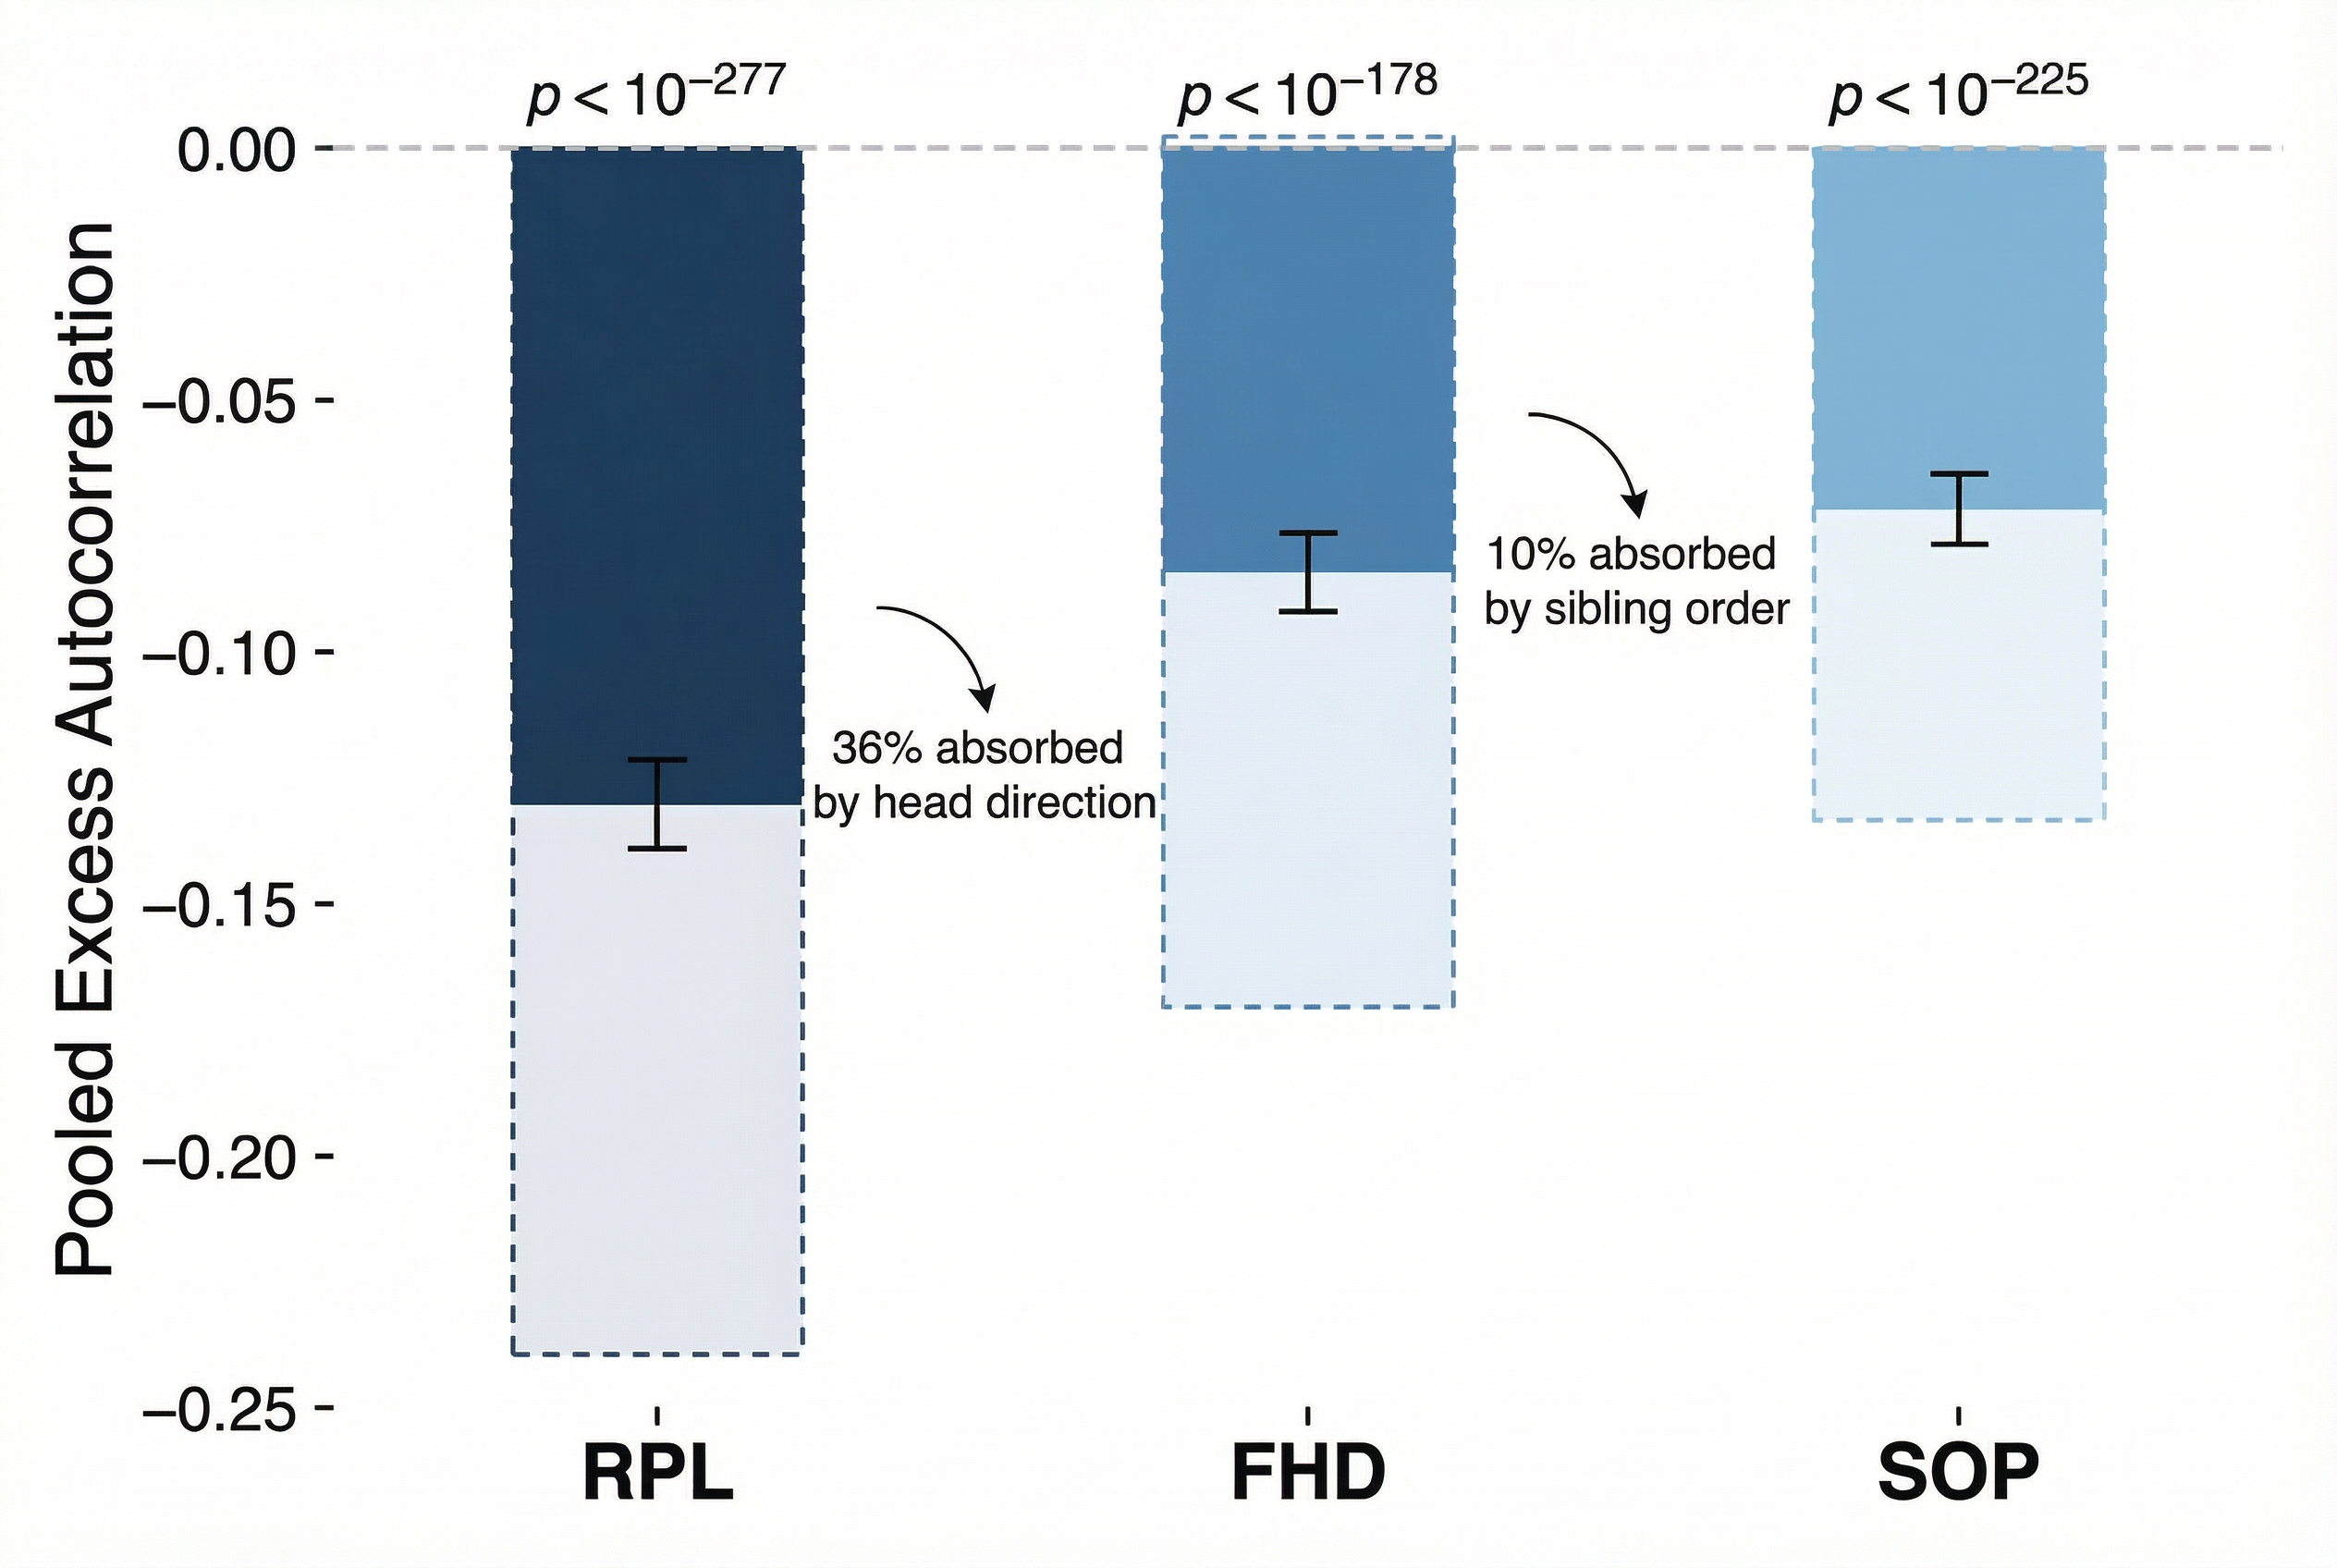
\includegraphics[width=0.85\textwidth,keepaspectratio]{figures/fig_4_v0.png}
  \caption{Pooled meta-analytic estimates of excess autocorrelation at three baseline tiers across 233 treebanks. The effect attenuates monotonically from excess-RPL ($-0.131$) through excess-FHD ($-0.084$) to excess-SOP ($-0.071$) as baselines incorporate more grammatical structure, but remains highly significant at all tiers. Error bars show 95\% confidence intervals; shaded bands show 95\% prediction intervals.}
  \label{fig:attenuation}
\end{figure}

Figure~\ref{fig:attenuation} displays the monotonic attenuation of compensatory anti-correlation through the three-tier baseline hierarchy.

\subsection{Phase 4--5: Typological Modulation}
\label{sec:typological}

\subsubsection{Case-Marking Richness}

The Spearman rank correlation between WALS Chapter 49A ordinal case-marking scale and UD-derived Case feature proportions is $\rho = 0.609$ ($p < 10^{-14}$), validating cross-source consistency while respecting the ordinal nature of the WALS scale.

Mixed-effects regression with language-family random intercepts ($N = 211$ treebanks with complete typological data) reveals that case-marking richness is a highly significant positive predictor of excess-RPL ($\beta = 0.080$, $SE = 0.017$, $p < 10^{-6}$): languages with richer morphological case systems show less negative (weaker) compensatory anti-correlation. The direction is consistent with the global morphology--word-order trade-off \citep{Bentz2017}: languages with richer case marking have more flexible word order and less need for sequential compensation of processing load.

When word-order typology (SVO, SOV, VSO) is added to the regression, both SVO ($\beta = -0.051$, $p < 10^{-5}$) and VSO ($\beta = -0.051$, $p = 0.015$) show significantly more negative excess than SOV languages. After controlling for word order, the case-marking coefficient is attenuated ($\beta = 0.012$, $p = 0.50$), suggesting that word-order typology mediates part of the case-marking effect --- consistent with the known correlation between word-order rigidity and case-marking richness \citep{Bentz2017}.

\begin{figure}[!htbp]
  \centering
  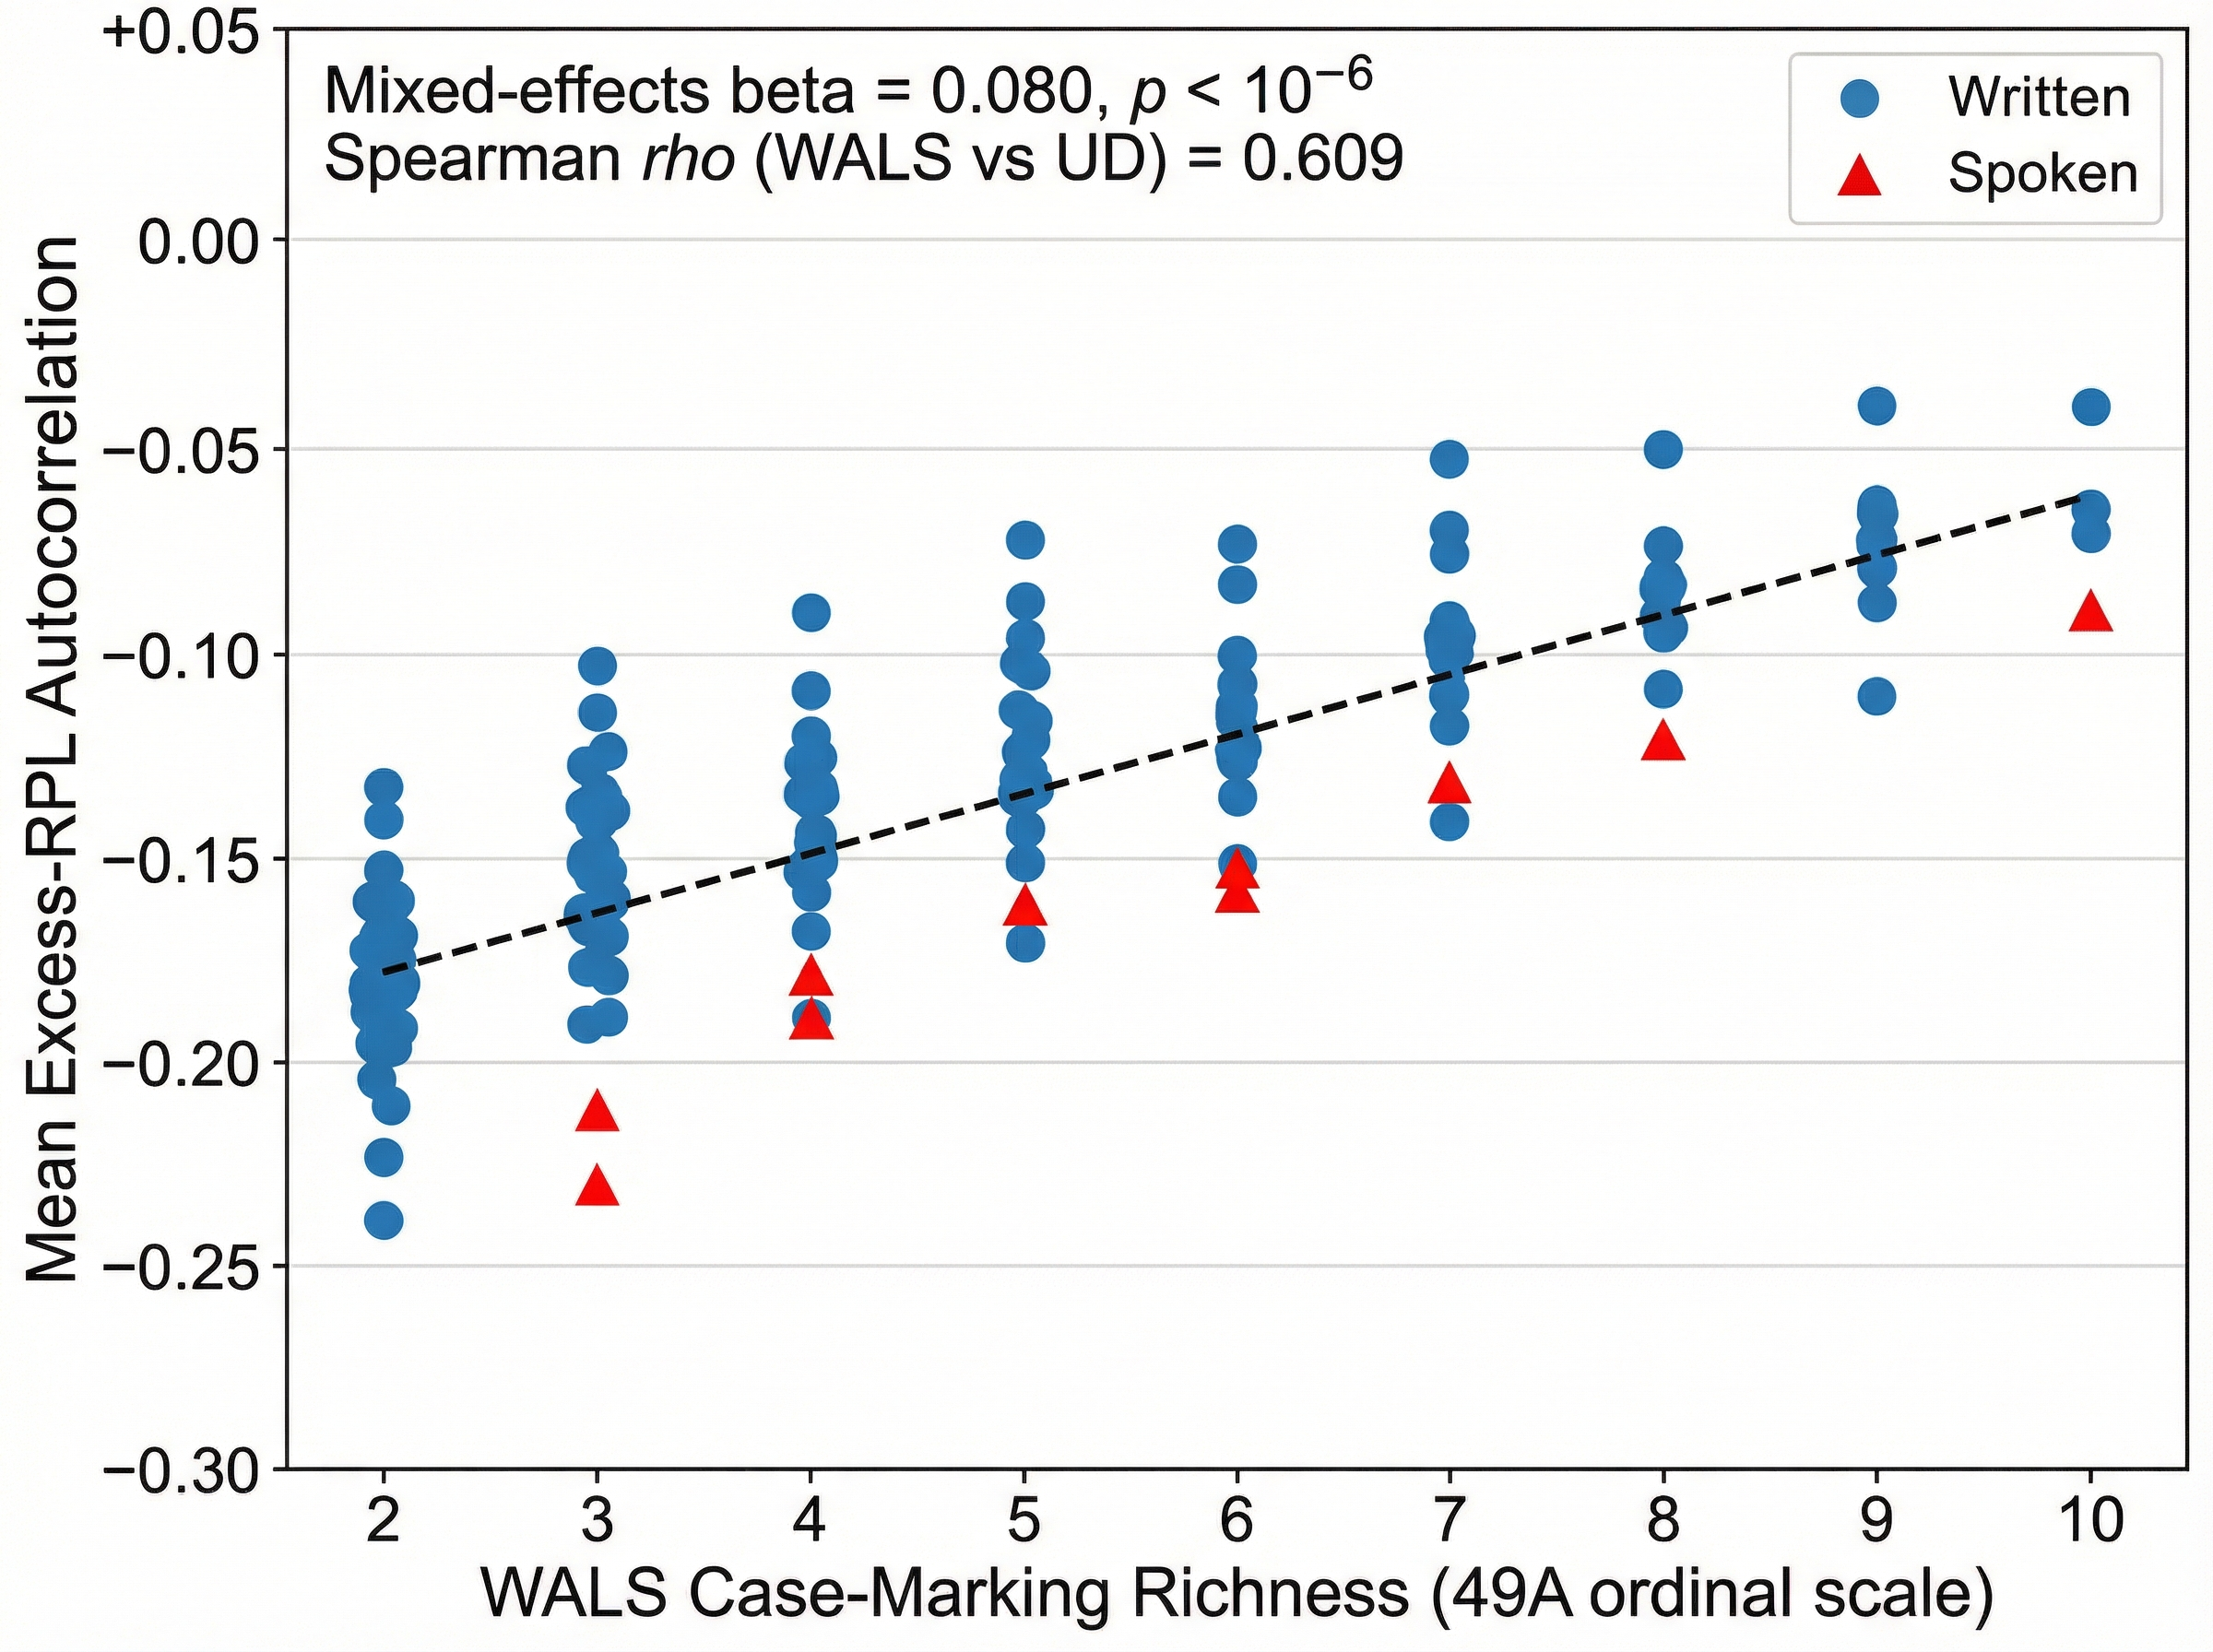
\includegraphics[width=0.85\textwidth,keepaspectratio]{figures/fig_5_v0.png}
  \caption{Relationship between morphological case-marking richness (WALS Chapter 49A ordinal scale) and mean excess-RPL autocorrelation across treebanks. Languages with richer case systems show less negative (weaker) compensatory anti-correlation ($\beta = 0.080$, $p < 10^{-6}$ in mixed-effects model with language-family random intercepts). Each point represents one treebank; color indicates modality (blue = written, red = spoken). Dashed line shows the OLS regression fit.}
  \label{fig:case_marking}
\end{figure}

Figure~\ref{fig:case_marking} visualizes the relationship between case-marking richness and anti-correlation strength, showing the predicted positive slope.

\subsubsection{Spoken vs.\ Written Modality}

Spoken treebanks ($n = 13$) show significantly more negative mean excess-RPL ($-0.167$) than written treebanks ($n = 198$, mean $= -0.129$), with a large effect size (Cohen's $d = -0.83$, $p = 0.001$). In the mixed-effects model controlling for language family and mean sentence length, the spoken coefficient remains significant ($\beta = -0.035$, $SE = 0.014$, $p = 0.014$).

The scope of the long-sentence restriction differs substantially by modality: the median proportion of sentences reaching $\geq 20$ tokens is 24.1\% for spoken treebanks versus 40.6\% for written treebanks. The qualifying long-sentence subset of spoken corpora thus represents a smaller and potentially less representative sample of spoken language production. The spoken/written comparison should be interpreted with this caveat --- the stronger anti-correlation in spoken treebanks applies specifically to syntactically complex spoken utterances, which constitute a minority of spoken output.

\subsection{Phase 6: Robustness Analyses}
\label{sec:robustness}

Four pipeline variants tested sensitivity to key analytical decisions across 50 typologically diverse treebanks with 100 RPL permutations per sentence:

\begin{table}[!htbp]
\centering
\caption{Robustness analysis: pooled excess-RPL across four pipeline variants (50 treebanks). All variants yield strongly significant negative excess.}
\label{tab:robustness}
\begin{tabular}{llccc}
\toprule
\textbf{Variant} & \textbf{Description} & \textbf{Pooled} & \textbf{$I^2$} & \textbf{Pred.\ Int.} \\
\midrule
A & Punct excl., $\geq 20$ tok. & $-0.207$ & 0.978 & $[-0.328, -0.087]$ \\
B & Punct incl., $\geq 20$ tok. & $-0.156$ & --- & --- \\
C & Punct excl., $\geq 15$ tok. & $-0.201$ & --- & --- \\
D & Projective only, $\geq 20$ tok. & $-0.207$ & --- & --- \\
\bottomrule
\end{tabular}
\end{table}

\textbf{Punctuation effect (A vs.\ B).} Including punctuation attenuates the excess by approximately 0.052 (Wilcoxon $p < 10^{-5}$), confirming that punctuation's systematically short distances at predictable positions partially mask genuine compensatory dynamics. The effect remains strongly significant with punctuation included ($-0.156$), but the cleaner signal emerges with punctuation excluded.

\textbf{Length threshold (A vs.\ C).} Lowering the threshold from $\geq 20$ to $\geq 15$ tokens produces only mild attenuation ($-0.207 \to -0.201$), confirming graceful degradation at shorter sentence lengths despite increased estimator noise.

\textbf{Projectivity (A vs.\ D).} Restricting to projective sentences yields virtually identical results ($-0.207$ vs.\ $-0.207$, $\Delta = -0.0003$), indicating that non-projective sentences neither inflate nor deflate the excess autocorrelation.

\begin{figure}[!htbp]
  \centering
  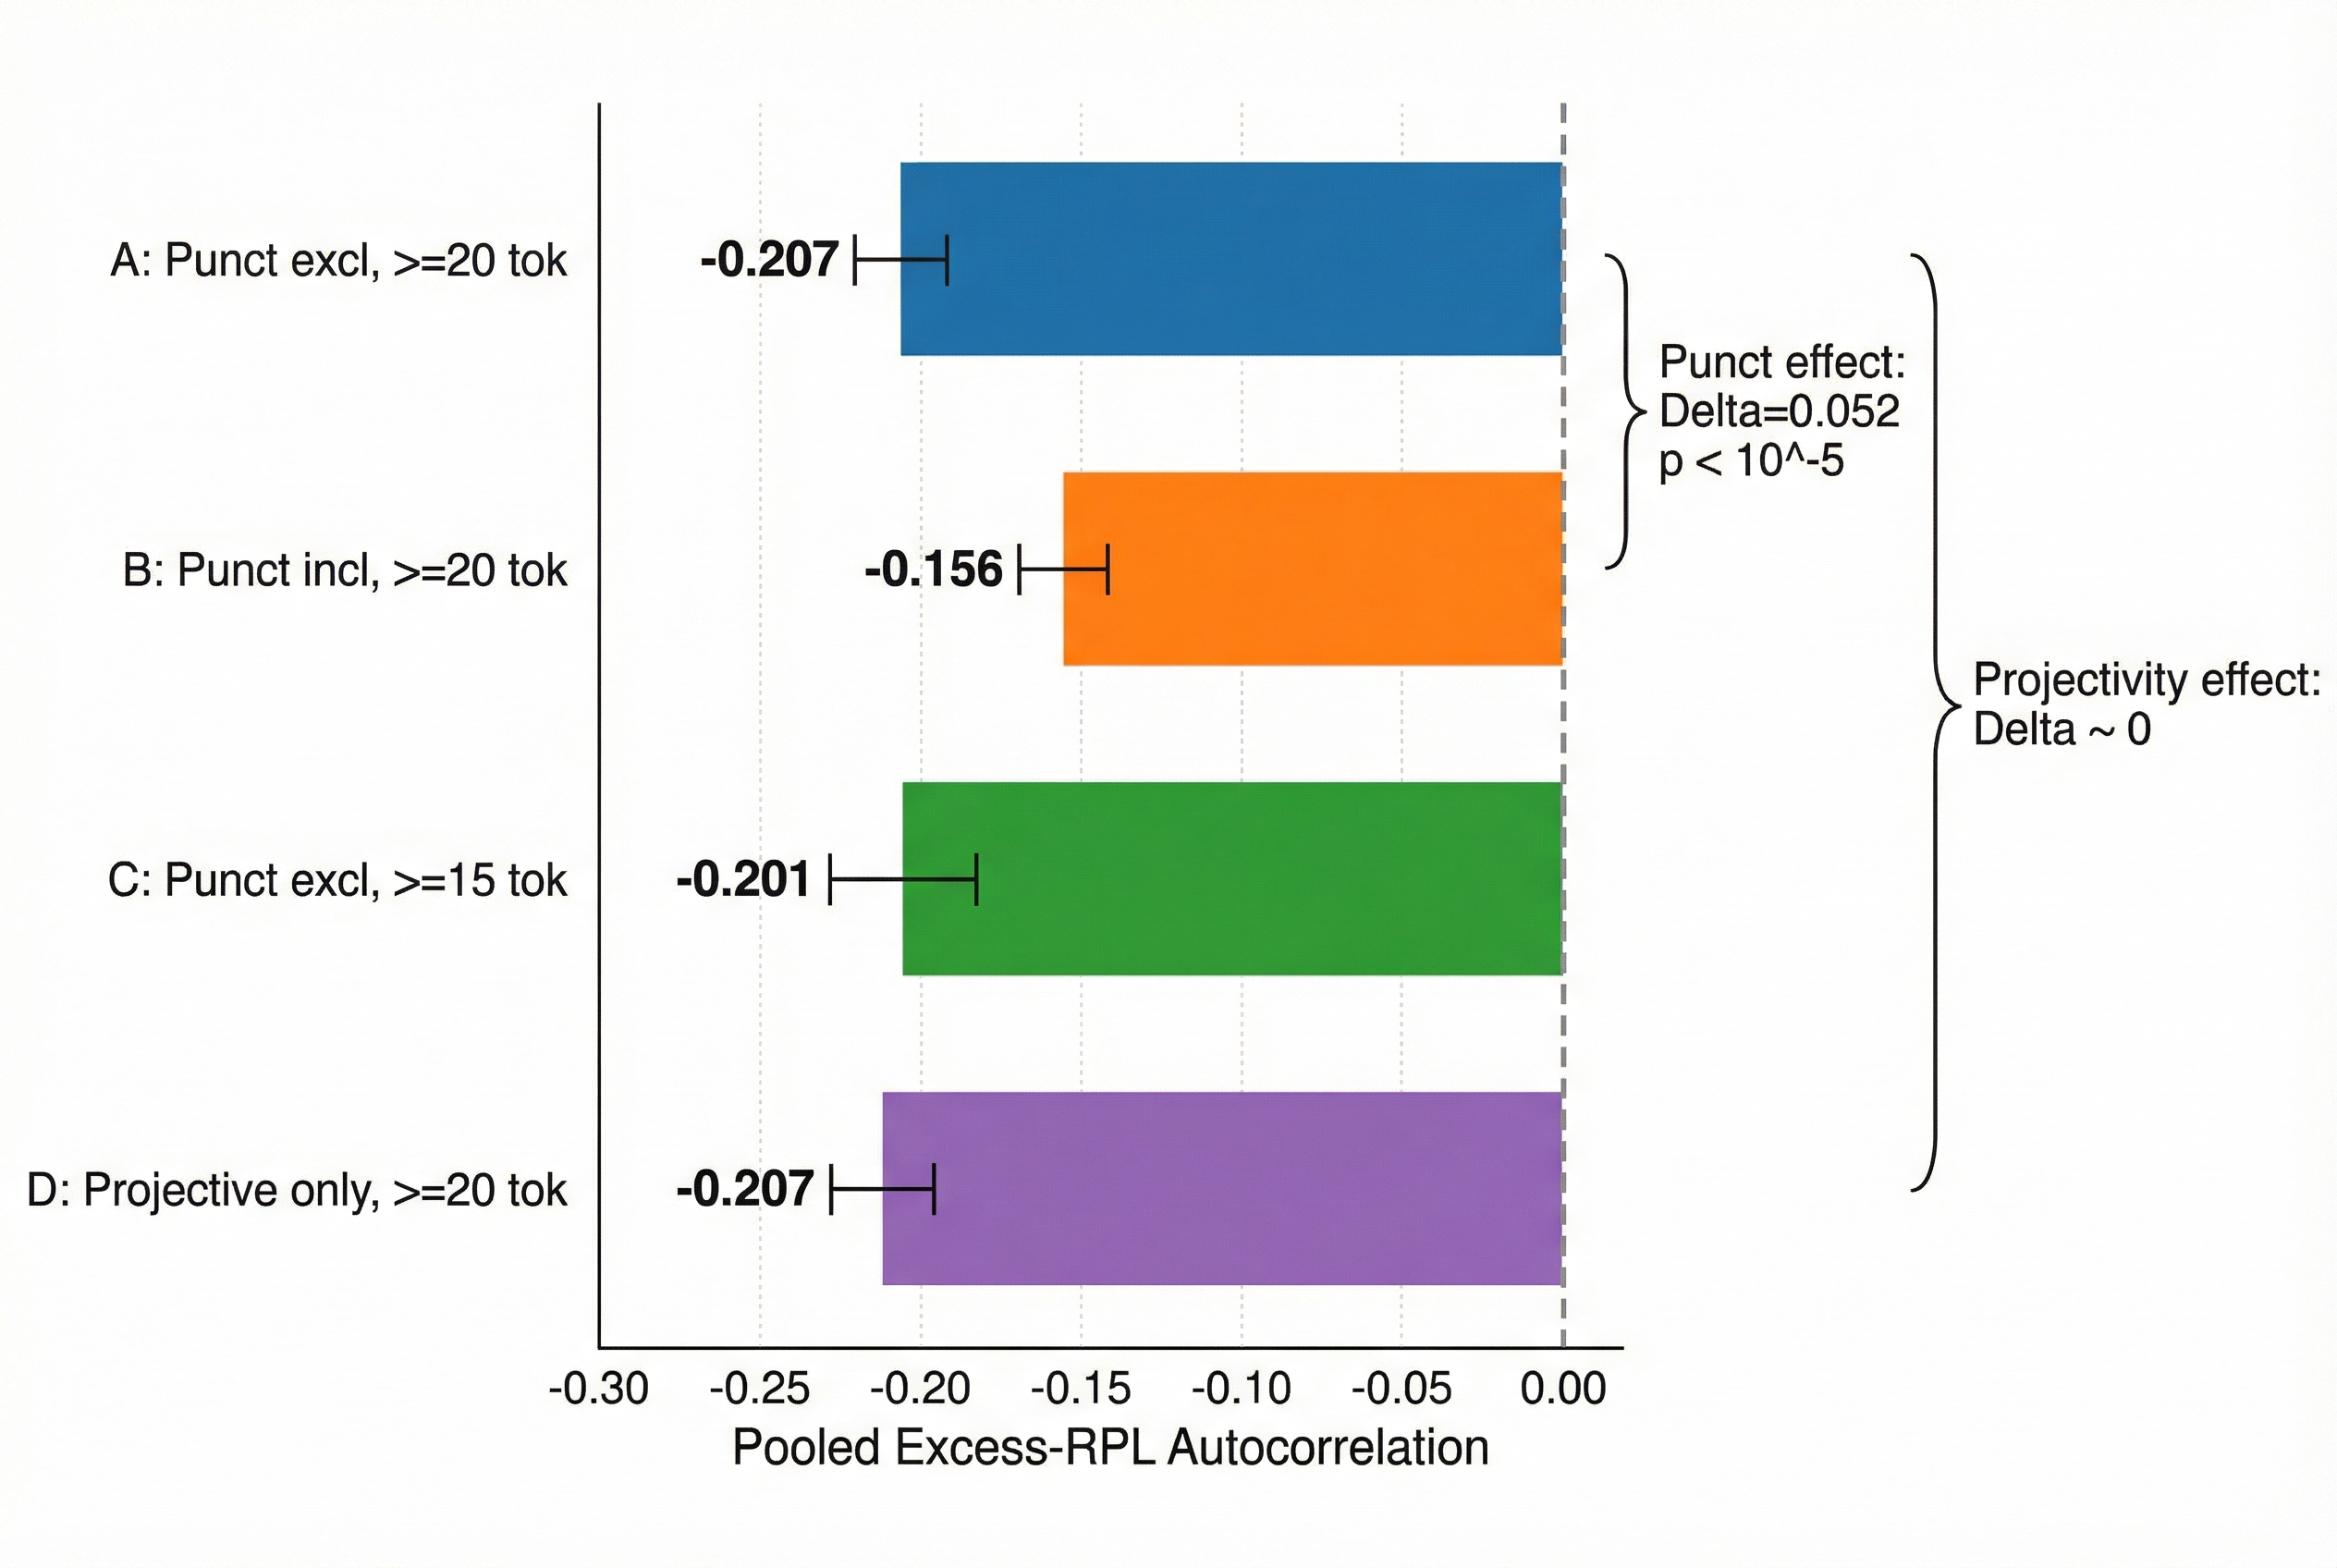
\includegraphics[width=0.85\textwidth,keepaspectratio]{figures/fig_6_v0.png}
  \caption{Pooled excess-RPL autocorrelation across four robustness variants (50 treebanks each). Punctuation exclusion (A vs.\ B) strengthens the measured effect; lowering the length threshold to $\geq 15$ tokens (C) produces mild attenuation; restricting to projective sentences (D) yields virtually identical results. All variants yield strongly significant negative excess.}
  \label{fig:robustness}
\end{figure}

Figure~\ref{fig:robustness} summarizes the robustness analysis results across all four pipeline variants.

\section{Discussion}

\subsection{Compensatory Anti-Correlation as a Cross-Linguistic Regularity}

The results establish compensatory anti-correlation as a robust cross-linguistic regularity in syntactically complex sentences. The pooled excess-RPL of $-0.131$ across 233 treebanks ($p < 10^{-277}$) indicates that dependency distance sequences exhibit substantially more negative lag-1 autocorrelation than tree structure alone predicts. The effect survives the full three-tier baseline hierarchy: excess-SOP remains $-0.071$ ($p < 10^{-225}$) after controlling for head-direction regularities and co-dependent ordering conventions. The 95\% prediction interval for excess-SOP lies entirely below zero ($[-0.134, -0.008]$), meaning that even in future treebanks from unsampled languages, negative excess is predicted.

The geometric confound analysis rules out tree topology as an explanation. Canonical tree types (star, caterpillar, balanced) produce zero or positive excess under RPL baselines, and the RPL-vs-RPL null on real sentences is centered at zero ($+0.001$, $p = 0.23$). The critical comparison --- observed vs.\ shuffled linearizations, both compared against RPL --- shows that the sequential ordering of real sentences contributes $-0.091$ of excess beyond what random token permutation produces ($p < 10^{-51}$). The compensatory pattern is a property of how languages order words, not of tree geometry.

\subsection{Relationship to DDM and UID}

Compensatory anti-correlation is distinct from both DDM and UID. DDM characterizes the central tendency of dependency distances (sentence-level means shorter than baselines), whereas compensatory anti-correlation characterizes their sequential dynamics (within-sentence ``rhythm'' of integration demands). The two phenomena are logically independent: a sentence could minimize mean dependency distance while exhibiting zero autocorrelation, or vice versa.

The distinction from UID is grounded in the empirical uncorrelatedness of dependency distance and surprisal \citep{Demberg2008}. UID predicts smoothing of information rate (surprisal), but dependency distance captures a different dimension of processing complexity --- structural integration cost rather than predictability. The three-tier baseline hierarchy provides finer-grained control than UID's counterfactual baselines \citep{Clark2023}, and the morphology-modulation prediction has no analogue in existing UID frameworks. The compensatory anti-correlation documented here may represent a structural-syntactic analogue of information-rate smoothing operating at the level of syntactic integration demands rather than lexical predictability.

\subsection{Morphological Modulation and the Complexity Trade-Off}

The finding that case-marking richness significantly weakens compensatory anti-correlation ($\beta = 0.080$, $p < 10^{-6}$) provides the first within-sentence statistical signature of the global morphology--word-order trade-off \citep{Bentz2017}. Languages with rich case systems can use morphological cues to signal grammatical relations, reducing reliance on positional adjacency and thus reducing the pressure for sequential compensation of integration demands. The attenuation of the case-marking coefficient when word-order typology is added ($\beta = 0.012$, $p = 0.50$) is consistent with mediation: case-rich languages tend to have flexible word order (e.g., SOV), and word-order type captures much of the variance that case-marking predicts.

The stronger anti-correlation in spoken treebanks ($d = -0.83$) aligns with the hypothesis that online processing pressures are more acute in speech production, where planning and articulation occur under tighter time constraints than in writing. However, the small number of qualifying spoken treebanks ($n = 13$) and the unrepresentative nature of $\geq 20$-token spoken utterances warrant caution.

\subsection{Limitations}

Several limitations constrain interpretation. First, the restriction to sentences of $\geq 20$ non-punctuation tokens means the regularity is demonstrated for syntactically complex utterances, not for all natural language. Across 233 treebanks, the median proportion of sentences reaching this threshold is 40.6\% for written and 24.1\% for spoken treebanks. The $\geq 15$-token robustness check shows graceful degradation ($-0.201$ vs.\ $-0.207$), suggesting the pattern extends to moderately complex sentences.

Second, the 233 treebanks are phylogenetically imbalanced, with Indo-European languages comprising 53\% of the sample. The language-family random intercept partially addresses this, and the language-level sensitivity analysis ($K = 114$ languages, pooled $= -0.133$) confirms the result is not driven by over-represented families.

Third, WALS case-marking coverage reaches only 47.0\% of treebanks. The UD-derived Case feature proportion provides supplementary coverage but measures a different construct: frequency of case-marked tokens in running text versus number of case distinctions in the paradigm. The Spearman correlation of $\rho = 0.609$ indicates moderate but imperfect agreement.

Fourth, the SOP baseline's near-determinism for frequent constructions means that excess-SOP primarily captures anti-correlation from configurations where the grammar permits ordering variation. For constructions with near-categorical ordering conventions, the SOP baseline collapses to a single linearization, making excess-SOP uninformative for those specific constructions.

Fifth, multiple theoretical accounts could explain compensatory anti-correlation without invoking a single mechanism: online processing compensation (working memory depletion after long dependencies favors subsequent short ones), grammatical optimization (grammars distribute processing load), or information-theoretic constraints (uniform syntactic complexity). Distinguishing among these accounts requires experimental evidence beyond the scope of the present corpus study.

\section{Conclusion}

This paper establishes compensatory anti-correlation --- excess negative lag-1 autocorrelation in dependency distance sequences --- as a cross-linguistic regularity in syntactically complex sentences. Across 233 Universal Dependencies treebanks (418,806 sentences, 38 language families), the pooled excess autocorrelation relative to RPL baselines is $-0.131$ ($p < 10^{-277}$), and the effect survives through the full baseline hierarchy to excess-SOP $= -0.071$ ($p < 10^{-225}$). Geometric confound analysis confirms the pattern is not an artifact of tree topology. Morphological case-marking richness significantly modulates the effect ($\beta = 0.080$, $p < 10^{-6}$), providing the first within-sentence statistical signature of the global morphology--word-order trade-off.

Future work includes: (a) extending the analysis to lag-2 and higher-order autocorrelation; (b) testing whether compensatory anti-correlation varies across syntactic construction types; (c) developing processing models that predict the observed anti-correlation from cognitive constraints; and (d) investigating whether surprisal sequences exhibit analogous sequential structure, directly testing the relationship between compensatory anti-correlation and UID.

\bibliographystyle{plainnat}
\bibliography{references}

\end{document}
